% Springer Nature (LNCS) conference template version of the report.
% Same content as main-ieee.tex; references use IEEE style as the guidelines require.
% Build: see README.md in this folder (pdflatex, bibtex, pdflatex, pdflatex).
\documentclass[runningheads]{llncs}
% Packages shared by both templates.
\usepackage{graphicx}
\usepackage{amsmath,amssymb}
\usepackage{booktabs}
\usepackage{tabularx}
\usepackage{multirow}
\usepackage{algorithm}
\usepackage{algpseudocode}
\usepackage{tikz}
\usetikzlibrary{arrows.meta,positioning,shapes.geometric,calc}
\usepackage{url}
\usepackage{textcomp}
\usepackage{xcolor}
\graphicspath{{figures/}}
\renewcommand{\algorithmicrequire}{\textbf{Input:}}

\usepackage[hidelinks]{hyperref}
% Single-column layout: wide floats are ordinary floats.
\newenvironment{widefigure}{\begin{figure}[t]}{\end{figure}}
\newenvironment{widetable}{\begin{table}[t]}{\end{table}}

% Let floats sit near their text on the smaller LNCS page.
\renewcommand{\topfraction}{0.95}
\renewcommand{\bottomfraction}{0.6}
\renewcommand{\textfraction}{0.05}
\renewcommand{\floatpagefraction}{0.75}
\setcounter{topnumber}{4}
\setcounter{totalnumber}{6}
\newlength{\covergap}\setlength{\covergap}{0.45cm}
\newcommand{\coverlogo}{5.5cm}

\begin{document}
% Cover page, shared by both templates (content from the project synopsis).
\begin{titlepage}
\centering
\vspace*{0.5\covergap}

\includegraphics[width=\coverlogo]{mit_logo.jpg}\par
\vspace{0.9\covergap}
{\Large\bfseries MANIPAL INSTITUTE OF TECHNOLOGY\par}
\vspace{0.15cm}
{\normalsize\itshape (A constituent unit of Manipal Academy of Higher Education)\par}
\vspace{0.5\covergap}
{\large\bfseries School of Computer Engineering\par}
\vspace{1.0\covergap}
{\large\bfseries MINI PROJECT REPORT\par}
\vspace{0.3\covergap}
{\large\bfseries Parallel Computer Architecture and Programming (CSE-3129)\par}
\vspace{1.0\covergap}
{\Large\bfseries Heterogeneous Parallelization of an Agent-Based\\[2pt] Limit Order Book Simulator Using CUDA, OpenMP, and MPI\par}
\vspace{1.2\covergap}
{\large\bfseries Submitted by:\par}
\vspace{0.4\covergap}
{\normalsize
\begin{tabular}{|l|c|c|}
\hline
\textbf{Name} & \textbf{Registration Number} & \textbf{Roll Number}\\
\hline
Abhisaar Gupta & 240962059 & 10\\
Devesh Khaitan & 240962031 & 3\\
Sohan Kar      & 240962358 & 23\\
Pratham Dobhal & 240962422 & 29\\
\hline
\end{tabular}\par}
\vfill
{\small Source code: \url{https://github.com/abhisaarguptaa/Stock-market-simulator-using-PCAP}\par}
\vspace{0.3\covergap}
{\small October 2026\par}
\end{titlepage}


\title{Heterogeneous Parallelization of an Agent-Based Limit Order Book Simulator Using CUDA, OpenMP, and MPI}
\titlerunning{Heterogeneous Parallel Limit Order Book Simulator}
\author{Abhisaar Gupta \and Devesh Khaitan \and Sohan Kar \and Pratham Dobhal}
\authorrunning{A. Gupta et al.}
\institute{School of Computer Engineering, Manipal Institute of Technology,\\
Manipal Academy of Higher Education, Manipal, India}

\maketitle

\begin{abstract}
Agent-based simulators of limit order book (LOB) markets reproduce how prices form from the orders
of many independent traders, but mainstream simulators run as single-threaded event loops and scale
poorly with the number of agents and instruments. The workload is not uniformly parallel: agents
decide independently, which suits a GPU, while price--time priority forces the orders of one
instrument to be matched one at a time. We implement a deterministic simulator with a three-tier
heterogeneous mapping (agent decisions in CUDA, matching parallelised across instruments with
OpenMP, and instruments distributed across MPI ranks) and measure where its performance limits lie.
Every back end produces a bit-identical trade log for a given seed, verified on 12 configurations
covering 1.29 million trades. On a Tesla T4 the decision kernel is about 85$\times$ faster than
two CPU threads, yet whole-tick speedup is bounded at 1.11--1.41$\times$ because matching takes
92--96\% of each tick. CUDA overtakes the multicore baseline at 4{,}000--16{,}000 agents. On a
16-thread laptop, matching speeds up only across instruments (0.90$\times$ with one instrument,
3.97$\times$ with 128); strong scaling peaks at 1.99$\times$ on 8 threads with an effective serial
fraction of 0.49. The simulated returns show heavy tails and volatility clustering. The results
show that order matching under price--time priority, and not the agent computation, is the scaling
bottleneck on every back end.

\keywords{Limit order book \and Agent-based simulation \and Heterogeneous computing \and CUDA \and OpenMP \and MPI \and Amdahl's law \and Reproducibility}
\end{abstract}

% Sections 1-3 and 5-9 (Introduction ... Algorithms). Shared by both templates.

\section{Introduction}
A financial exchange is, at its core, a large concurrent system. Thousands of independent
participants form intentions at the same time, but their orders must be serialised into a single,
strictly ordered book per traded instrument before any trade can occur. Agent-based models (ABMs)
of limit order book (LOB) markets reproduce this structure in software and are widely used to study
price formation, liquidity, and the statistical regularities of returns~\cite{cont2001,preis2006}.
Their main practical limitation is computational: fidelity improves with the number of simulated
agents and instruments, yet mainstream market simulators execute as single-threaded discrete-event
loops~\cite{byrd2020abides} and therefore scale poorly with either.

This workload is interesting for a parallel computer architecture study because it is not
uniformly parallel. The agent decision phase is massively data-parallel and maps naturally onto a
GPU, since every agent independently reads a shared view of the book and emits at most one order.
The matching phase is the opposite: price--time priority imposes a total order on events within an
instrument, so matching for a single instrument resists parallelisation almost entirely and can
only be distributed across instruments. The simulation therefore contains an irreducible serial
core between two parallel regions, and the achievable speedup is governed by the interaction
between them rather than by the efficiency of any single kernel.

This project implements such a simulator with a three-tier heterogeneous mapping: agent decisions
in CUDA, per-instrument matching parallelised across instruments with OpenMP, and instrument sets
distributed across processes with MPI. We treat the resulting performance envelope as the object
of study. The main contributions are:
\begin{itemize}
\item A deterministic LOB simulator whose serial, OpenMP, CUDA and MPI back ends produce
  bit-identical trade logs for a given seed, verified by an order-sensitive hash of every trade.
\item Measurements of the CPU--GPU boundary cost, the effect of warp divergence and copy-back
  compaction, and the agent count at which heterogeneous execution overtakes a multicore baseline.
\item A strong, weak and per-instrument scaling study with Amdahl, Gustafson, Karp--Flatt and
  roofline analysis, showing that order matching is the bottleneck on every back end.
\item An open-source implementation with one-command setup and demo scripts, so every result in
  this report can be reproduced.
\end{itemize}

The rest of the report is organised as follows. Section~\ref{sec:lit} reviews related work,
Sections~\ref{sec:problem} and~\ref{sec:obj} state the problem and objectives,
Sections~\ref{sec:method}--\ref{sec:algo} describe the method, architecture and algorithms,
Sections~\ref{sec:setup}--\ref{sec:perf} present the experiments, results and analysis,
Section~\ref{sec:compare} compares the work with existing methods, and
Sections~\ref{sec:concl}--\ref{sec:future} conclude.

% Section 2: Literature Review. Shared by both templates.
\section{Literature Review}\label{sec:lit}

\subsection{Foundations}
Gode and Sunder showed that agents with no intelligence beyond a budget constraint already produce
near-efficient allocations in a double auction, so much of market behaviour comes from the trading
mechanism itself~\cite{gode1993}. Chiarella and Iori added fundamentalist, chartist and noise
traders interacting through an explicit order book~\cite{chiarella2002}; Preis et al.\ showed that a
simple multi-agent order book with price--time priority reproduces fat tails once order placement
depth depends on the trend~\cite{preis2006}; and Farmer et al.\ found that zero-intelligence order
flow explains much of the observed spread and price impact~\cite{farmer2005}. Cont's stylised facts
(heavy tails, volatility clustering and no linear autocorrelation) are the standard checklist for
validating such models~\cite{cont2001}. On the computing side, Lysenko and D'Souza built the first
largely GPU-resident ABM framework~\cite{lysenko2008}, Fujimoto surveyed parallel discrete-event
simulation~\cite{fujimoto1990}, and Amdahl~\cite{amdahl1967}, Gustafson~\cite{gustafson1988},
Karp and Flatt~\cite{karp1990} and Williams et al.~\cite{williams2009} give the performance models
used in this report.

\subsection{Recent agent-based market simulators}
\textbf{ABIDES-Gym}~\cite{amrouni2021} (ACM ICAIF 2021) wraps ABIDES~\cite{byrd2020abides}, a
message-driven discrete-event simulator with a NASDAQ-like exchange and price--time priority, as an
OpenAI Gym environment for reinforcement learning. It offers high fidelity and realistic latency,
but its kernel is a single-threaded event loop and the paper reports no run times; a later study
cites ABIDES at about 29{,}000 messages per second~\cite{mascioli2024}.

\textbf{JAX-LOB}~\cite{frey2023} (ACM ICAIF 2023) is the first GPU-accelerated LOB simulator. Each
book is a fixed-capacity array, and matching runs inside a JAX loop. The authors note that
processing messages within one book is inherently serial, so all parallelism comes from running
thousands of independent books with \texttt{vmap}: with 1000 books, a message costs about
2.6\,$\mu$s per book on an RTX 2080 Ti, and RL training is about 7$\times$ faster. Its limits are
pre-allocated capacity, a cost set by the slowest branch, and replayed order flow that does not
react to the agent. It does not measure the end-to-end serial fraction or combine GPU agents with
CPU matching.

\textbf{PyMarketSim}~\cite{mascioli2024} (ACM ICAIF 2024) is a Python discrete-time simulator whose
tick (observe, act, clear, advance) matches ours. Its order book takes 1.9--4.7\,$\mu$s per
operation from $10^3$ to $10^6$ orders, about 300{,}000 book operations or 15{,}000 agent actions
per second, but it is serial, simulates one asset and uses 25 agents in its experiments.

\subsection{GPU and high-performance ABM frameworks}
\textbf{FLAME GPU 2}~\cite{richmond2023} (Software: Practice and Experience 2023) compiles agent
functions to CUDA at run time, stores agents as structures of arrays, and passes messages through
spatial, array or bucket structures. It runs up to 200 million agents on a V100 and 1M agents in
about 3\,ms per step. Its performance depends on spatial or keyed locality; agents competing for
one resource need repeated bidding sub-models, atomics are non-deterministic, and one model is
limited to one GPU.

\textbf{Agents.jl}~\cite{datseris2024} (SIMULATION 2024, online 2022) is a Julia ABM library that
runs single models about 2--125$\times$ faster than MASON, NetLogo and Mesa in the authors'
benchmarks. It does not parallelise within a model, because agents mutate shared state, and has no
GPU support: the same shared-state conflict that an order book creates.

\subsection{Matching engines and hardware-accelerated trading}
\textbf{CoinTossX}~\cite{jericevich2022} (SoftwareX 2022) is an open-source Java matching engine
modelled on the Johannesburg Stock Exchange, with price--time priority and messaging over UDP. It
reaches 106--248\,ns 90th-percentile matching latency on a 16-core server, but throughput falls from
2{,}287 to 621--989 orders per second as client--stock pairs are added, and it is engineered for
latency rather than for parallel scaling.

\textbf{LightTrader}~\cite{yoo2023} (IEEE HPCA 2023) is a heterogeneous high-frequency trading system:
an FPGA parses market data and keeps the top of a local order book, while custom deep-learning
accelerators run price-prediction models, with a scheduler that picks batch size and voltage and
frequency under a power budget. It is 13.9$\times$ faster than a V100-based system for AI
processing, but scaling saturates as accelerators share the power budget. It accelerates the
\emph{decision} stage for one trader, the analogue of our GPU phase.

\subsection{Distributed ABM and reproducible parallel random numbers}
\textbf{Repast4Py}~\cite{collier2022} (Winter Simulation Conference 2022) distributes Python ABMs
with MPI, partitioning space across ranks with ghost regions. A 3.6M-agent random walk speeds up
4.39$\times$ from 36 to 288 ranks (efficiency 0.94 to 0.55), while a network model reaches only
1.75$\times$ (efficiency 0.22): communication dominates at higher rank counts. Whether results are
identical across rank counts is not addressed.

\textbf{SIMCoV-GPU}~\cite{leyba2024} (ACM HPDC 2024) ports a spatial infection ABM to multiple GPUs
with CUDA and UPC++, reaching 11.9$\times$ over 512 CPU cores with 16 GPUs. The GPU wins only on
large enough problems (at 64 GPUs on a small grid it is 0.85$\times$), and because CPU and GPU
random number generators differ, results agree only statistically (within about 1\%), not bit for
bit.

\textbf{OpenRAND}~\cite{khan2024} (SoftwareX 2024) provides counter-based generators (Philox,
Threefry and others) keyed by a logical entity rather than a thread, so streams give the same
output on any thread count or device; it is 1.8$\times$ faster than cuRAND in a particle
benchmark. It supplies reproducible random numbers but not reproducibility of a whole simulation,
which also needs deterministic arithmetic and event ordering.

\subsection{Summary, research gaps and motivation}
Table~\ref{tab:lit} summarises the reviewed work. Four gaps motivate this project:
\begin{enumerate}
\item \textbf{Market simulators are built for fidelity, not parallel characterisation.}
  ABIDES-Gym, PyMarketSim and CoinTossX run essentially serially; JAX-LOB parallelises only across
  independent books. None splits the tick into a parallel decision phase and a serial matching
  phase and relates the measured speedup to Amdahl's law.
\item \textbf{The serial matching core is acknowledged but not measured.} No study reports what
  share of tick time matching takes as agents grow, or the gap between kernel and end-to-end
  speedup.
\item \textbf{GPU and distributed ABM frameworks rely on locality.} FLAME GPU 2, Repast4Py and
  SIMCoV-GPU exploit spatial neighbourhoods and halos; Agents.jl avoids in-model parallelism. An
  order book, where every agent writes into one strictly ordered structure per instrument, fits
  none of them.
\item \textbf{Bit-identical heterogeneous results are rare.} SIMCoV-GPU accepts statistical
  agreement and FLAME GPU 2 has non-deterministic atomics; OpenRAND makes only the random numbers
  reproducible. No reviewed work shows a bit-identical event log across CUDA, OpenMP and MPI.
\end{enumerate}
We therefore build a simulator that partitions by instrument, keeps the GPU for decisions only,
produces identical trades on every back end, and measures where its speedup stops and why.

\begin{widetable}
\centering
\caption{Comparison of recent related work (2021--2024).}
\label{tab:lit}
\footnotesize
\begin{tabularx}{\textwidth}{@{}p{2.3cm} X X X p{2.0cm}@{}}
\toprule
Work & Approach / platform & Advantages & Limitations & Key result\\
\midrule
ABIDES-Gym~\cite{amrouni2021} & discrete-event kernel, Python, serial & high fidelity, latency model, RL interface & single-threaded; no run times reported & --\\
JAX-LOB~\cite{frey2023} & JAX on GPU, \texttt{vmap} over books & thousands of books in parallel; RL on GPU & serial within a book; fixed capacity & 2.6\,$\mu$s/msg per book; 7$\times$ RL\\
PyMarketSim~\cite{mascioli2024} & Python discrete-time tick & simple, RL and game-theory tools & serial; one asset; 25 agents & 300k book ops/s\\
FLAME GPU 2~\cite{richmond2023} & CUDA, SoA, spatial messages & 200M agents on one GPU & needs locality; non-det.\ atomics; 1 GPU per model & 1M agents in 3\,ms/step\\
Agents.jl~\cite{datseris2024} & Julia, CPU & concise and fast single models & no in-model parallelism; no GPU & 2--125$\times$ vs other ABM tools\\
CoinTossX~\cite{jericevich2022} & Java engine, UDP & sub-$\mu$s matching latency & throughput falls with instruments & 106--248\,ns latency\\
LightTrader~\cite{yoo2023} & FPGA + DL accelerators & fast decision stage, energy-aware & power-limited scaling; one trader & 13.9$\times$ vs V100 system\\
Repast4Py~\cite{collier2022} & Python + MPI, spatial partitions & HPC scale from Python & communication-bound at high rank counts & 4.39$\times$, 36$\to$288 ranks\\
SIMCoV-GPU~\cite{leyba2024} & CUDA + UPC++, multi-GPU & 11.9$\times$ over 512 cores & GPU wins only at large sizes; not bitwise reproducible & 11.9$\times$ (16 GPUs)\\
OpenRAND~\cite{khan2024} & counter-based RNG library & reproducible on any back end & RNG only, not whole simulation & 1.8$\times$ vs cuRAND\\
\bottomrule
\end{tabularx}
\end{widetable}


\section{Problem Statement}\label{sec:problem}
Given a population of $N$ heterogeneous trading agents and $M$ instruments, each with its own
limit order book, simulate $T$ discrete ticks in which (i) every agent observes a snapshot of its
instrument's book and may submit, cancel or modify one order, (ii) each instrument's orders are
matched under price--time priority, and (iii) a market-wide index is published for the next tick.
The problem is to map this pipeline onto heterogeneous hardware (a GPU, a multicore CPU and
multiple processes) such that:
\begin{enumerate}
\item the parallel versions produce \emph{exactly} the same trades as a serial reference for the
  same random seed, so that correctness can be checked and experiments repeated;
\item the speedup over the serial reference is measured and explained, including the serial
  fraction imposed by price--time priority, the cost of moving data across the CPU--GPU boundary,
  and the cost of synchronising MPI ranks at every tick; and
\item the agent and instrument counts at which the heterogeneous mapping beats an optimised
  multicore CPU implementation are identified.
\end{enumerate}
The simulated market must also remain realistic, reproducing the standard stylised facts of
financial returns~\cite{cont2001}.

\section{Objectives}\label{sec:obj}
The eight objectives from the project synopsis, and where each is addressed, are:
\begin{enumerate}
\item \textbf{Serial matching engine.} Implement a correct serial LOB engine supporting add,
  cancel, modify and market orders under price--time priority, with a unit test suite as the
  correctness reference (Sections~\ref{sec:method}, \ref{sec:algo}, \ref{sec:res-correct}).
\item \textbf{Agents and serial baseline.} Implement noise, momentum, mean-reverting and
  market-making agents and a fully serial simulator as the speedup baseline
  (Section~\ref{sec:method}).
\item \textbf{CUDA agent phase.} Port agent decisions to CUDA with agent-type sorting to reduce warp
  divergence, coalesced access, and counter-based random streams for determinism
  (Sections~\ref{sec:algo}, \ref{sec:res-gpu}).
\item \textbf{OpenMP matching.} Parallelise matching across instruments and evaluate thread scaling,
  false sharing and memory contention (Section~\ref{sec:res-cpu}).
\item \textbf{MPI distribution.} Distribute instruments across ranks with a per-tick index reduction
  and quantify communication overhead (Section~\ref{sec:res-cpu}).
\item \textbf{Validation.} Compare trade logs exactly across back ends and check the stylised facts
  (Sections~\ref{sec:res-correct}, \ref{sec:res-facts}).
\item \textbf{Scaling study.} Strong and weak scaling, an Amdahl fit of the serial fraction,
  roofline placement and Nsight metrics (Sections~\ref{sec:results}, \ref{sec:perf}).
\item \textbf{CPU vs GPU threshold.} Identify where the heterogeneous mapping overtakes the
  multicore CPU and explain why (Sections~\ref{sec:res-gpu}, \ref{sec:perf}).
\end{enumerate}

\section{Proposed Methodology}\label{sec:method}

\subsection{Barrier-synchronised tick}
The simulator advances in discrete ticks. Following the conservative synchronisation family of
parallel discrete-event simulation~\cite{fujimoto1990}, every tick has three phases separated by
barriers:
\begin{enumerate}
\item \textbf{Decide} (parallel over agents): each agent reads its instrument's snapshot (best bid,
  best ask, last price, trend) and the market index, and emits at most one order intent.
\item \textbf{Match} (parallel over instruments, serial inside each): the intents of each instrument
  are applied to its book in a deterministic arrival order, producing trades.
\item \textbf{Publish} (reduction over instruments): snapshots for the next tick are rebuilt and the
  market index (the sum of mid prices) is reduced, across ranks with \texttt{MPI\_Allreduce}.
\end{enumerate}
This trades some concurrency for determinism and auditability; the cost of the barrier is one of
the quantities measured.

\subsection{Order book}
Each instrument has a fixed grid of 4096 integer price levels with one FIFO queue per level. Orders
live in a node pool and are doubly linked into their level, with an id-to-node hash map, so add,
cancel and modify are $O(1)$ except for moving the best-price pointer when a level empties. Limit
orders match against the opposite side at the resting (maker) price and the remainder rests;
market orders match and drop any unfilled remainder. A modify keeps time priority only for a
quantity decrease at the same price. Resting orders expire after a time-to-live (100 ticks by
default), which keeps the book bounded.

\subsection{Agent population}
Four strategies, after the heterogeneous populations of~\cite{chiarella2002,preis2006}, are written
once as \texttt{\_\_host\_\_ \_\_device\_\_} functions so that the CPU loops and the CUDA kernel run
literally the same code (Table~\ref{tab:agents}). Agents are stateless functions of (agent id,
tick, seed, snapshot): they do not track inventory, which keeps the GPU phase free of per-tick
feedback from the matching engine.

\begin{table}[t]
\centering
\caption{Agent population (default mix).}
\label{tab:agents}
\footnotesize
\begin{tabularx}{\columnwidth}{@{}l c c X@{}}
\toprule
Strategy & Share & Acts/tick & Behaviour\\
\midrule
Noise & 65\% & 10\% & random side; mostly limit orders near the reference price\\
Momentum & 15\% & 5\% & market order in the direction of the instrument and index trend\\
Mean-reverting & 10\% & 3\% & limit order back toward the fundamental value\\
Market maker & 10\% & 100\% & re-quotes one side per tick, cancels its quote from two ticks earlier\\
\bottomrule
\end{tabularx}
\end{table}

\subsection{Determinism by design}
Parallel stochastic simulations are usually not repeatable, because random draws and floating-point
reductions depend on thread scheduling. We make every back end produce the identical trade log:
\begin{itemize}
\item \textbf{Counter-based RNG:} Philox4x32-10~\cite{salmon2011} maps (seed, stream, agent, tick)
  to random numbers with no shared state, so thread order cannot change any draw.
\item \textbf{Integer-only decisions:} CPU and GPU floating point can round differently (fused
  multiply--add, math libraries), so decisions use integer arithmetic.
\item \textbf{Deterministic arrival order:} intents are applied in agent-id order, rotated by a
  random offset per (instrument, tick) so that no agent is always first.
\item \textbf{Predictable order ids:} an order's id is $(\textit{tick}+1)\ll 32 \mid \textit{agent}$,
  so a market maker on the GPU can cancel its earlier quote without feedback from the CPU.
\item \textbf{Integer reductions:} the index is a sum of integers, so \texttt{MPI\_Allreduce} gives
  the same result in any reduction order.
\item \textbf{Order-independent compaction:} GPU output slots are reserved with
  \texttt{atomicAdd}; each entry carries its agent index and the host scatters by index.
\end{itemize}
Correctness is checked with an order-sensitive FNV-1a hash over every trade (tick, price,
quantity, buyer, seller, maker and taker ids), combined across instruments and ranks.

\subsection{Parallel mapping}
\begin{itemize}
\item \textbf{CUDA (decide):} one thread per agent, structure-of-arrays layout for coalesced loads,
  agents sorted by strategy so that warps mostly take one branch, snapshots read through the
  read-only cache (\texttt{\_\_ldg}), parameters in constant memory, and compaction of the copy
  back to only the agents that acted (about 20\% per tick).
\item \textbf{OpenMP (decide and match):} \texttt{parallel for schedule(static)} over agents for decisions;
  \texttt{parallel for schedule(dynamic,1)} over instruments for matching, with per-thread counters
  padded to 64-byte cache lines to avoid false sharing.
\item \textbf{MPI (instruments):} each rank owns a contiguous block of instruments and the agents
  trading them; ranks meet once per tick in an integer \texttt{MPI\_Allreduce}.
\end{itemize}

\subsection{Measurement}
The program times every phase of every tick (decide, host-to-device copy, kernel, device-to-host
copy, match, publish, MPI communication) and reports totals; for MPI it reports the slowest rank.
Kernel time uses CUDA events. Speedup is $S(p)=T_1/T_p$ against the serial back end, efficiency
is $E(p)=S(p)/p$, the serial fraction $f$ is fitted to Amdahl's law
$S(p)=1/(f+(1-f)/p)$~\cite{amdahl1967} by least squares, and the Karp--Flatt metric
$e(p)=(1/S-1/p)/(1-1/p)$~\cite{karp1990} is reported for each $p$. Weak scaling is interpreted
with Gustafson's law~\cite{gustafson1988} and the kernel is placed on a roofline~\cite{williams2009}
from Nsight Compute counters.

\section{System Architecture}\label{sec:arch}
Fig.~\ref{fig:arch} shows how the three tiers map onto hardware and Fig.~\ref{fig:flow} shows the
control flow of one simulation run. MPI splits the instruments into blocks, one per rank. Inside a
rank, the decision phase runs on the GPU (or on all CPU cores with OpenMP), and the matching phase
runs on the CPU with one instrument per OpenMP thread at a time. The ranks synchronise once per
tick to reduce the market index. Table~\ref{tab:modules} lists the software modules.

\begin{figure}[t]
\centering
\resizebox{\columnwidth}{!}{%
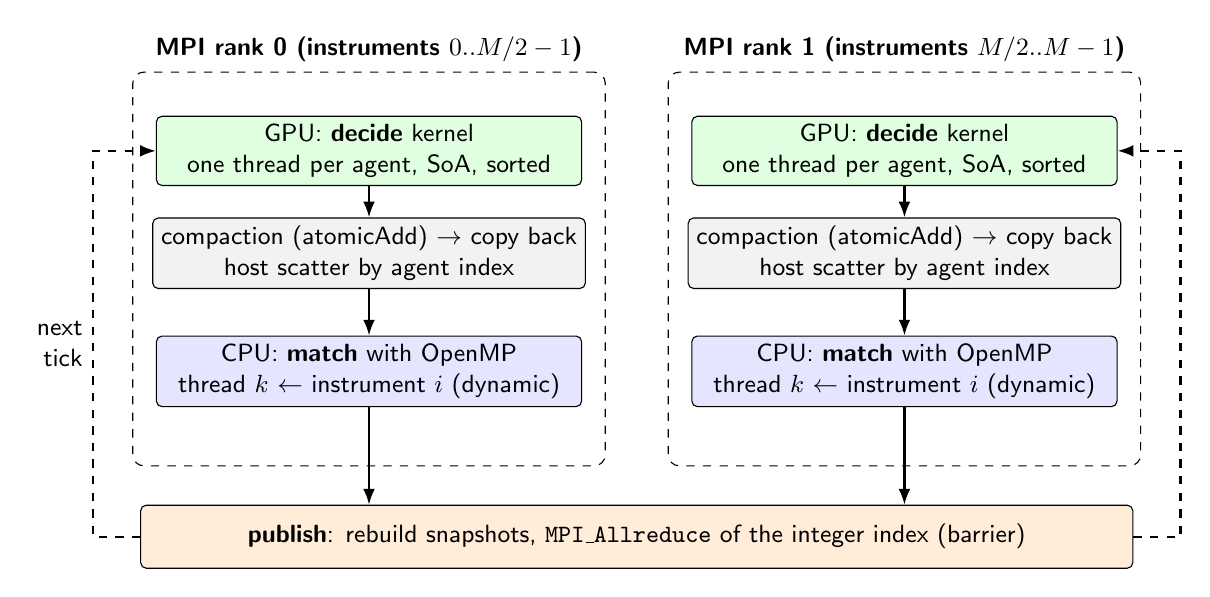
\begin{tikzpicture}[
  font=\sffamily\small,
  box/.style={draw, rounded corners=2pt, align=center, minimum height=0.8cm, inner sep=3pt},
  gpu/.style={box, fill=green!12},
  cpu/.style={box, fill=blue!10},
  net/.style={box, fill=orange!15},
  arr/.style={-{Latex[length=2mm]}, thick}]
  % Rank 0
  \node[draw, dashed, rounded corners, minimum width=6.0cm, minimum height=5.0cm,
        label={[font=\sffamily\bfseries\small]above:MPI rank 0 (instruments $0..M/2-1$)}] (r0) at (0,0) {};
  \node[gpu, minimum width=5.4cm] (g0) at (0,1.5) {GPU: \textbf{decide} kernel\\one thread per agent, SoA, sorted};
  \node[box, minimum width=5.4cm, fill=gray!10] (c0) at (0,0.2) {compaction (atomicAdd) $\rightarrow$ copy back\\host scatter by agent index};
  \node[cpu, minimum width=5.4cm] (m0) at (0,-1.3) {CPU: \textbf{match} with OpenMP\\thread $k$ $\leftarrow$ instrument $i$ (dynamic)};
  \draw[arr] (g0) -- (c0); \draw[arr] (c0) -- (m0);
  % Rank 1
  \node[draw, dashed, rounded corners, minimum width=6.0cm, minimum height=5.0cm,
        label={[font=\sffamily\bfseries\small]above:MPI rank 1 (instruments $M/2..M-1$)}] (r1) at (6.8,0) {};
  \node[gpu, minimum width=5.4cm] (g1) at (6.8,1.5) {GPU: \textbf{decide} kernel\\one thread per agent, SoA, sorted};
  \node[box, minimum width=5.4cm, fill=gray!10] (c1) at (6.8,0.2) {compaction (atomicAdd) $\rightarrow$ copy back\\host scatter by agent index};
  \node[cpu, minimum width=5.4cm] (m1) at (6.8,-1.3) {CPU: \textbf{match} with OpenMP\\thread $k$ $\leftarrow$ instrument $i$ (dynamic)};
  \draw[arr] (g1) -- (c1); \draw[arr] (c1) -- (m1);
  % Allreduce
  \node[net, minimum width=12.6cm] (ar) at (3.4,-3.4) {\textbf{publish}: rebuild snapshots, \texttt{MPI\_Allreduce} of the integer index (barrier)};
  \draw[arr] (m0) -- (m0|-ar.north); \draw[arr] (m1) -- (m1|-ar.north);
  \draw[arr, dashed] (ar.west) -- ++(-0.6,0) |- node[pos=0.25, left, align=right]{next\\tick} (g0.west);
  \draw[arr, dashed] (ar.east) -- ++(0.6,0) |- (g1.east);
\end{tikzpicture}}
\caption{System architecture: the three-tier heterogeneous mapping (two MPI ranks shown).}
\label{fig:arch}
\end{figure}

\begin{figure}[t]
\centering
\resizebox{0.86\columnwidth}{!}{%
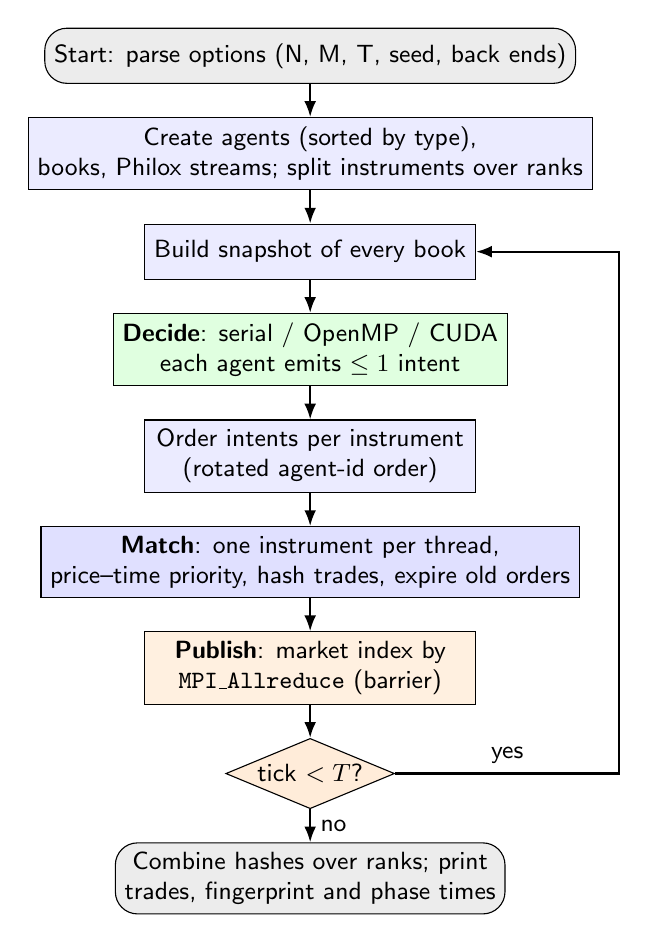
\begin{tikzpicture}[
  font=\sffamily\small, node distance=0.42cm,
  st/.style={draw, rounded corners=8pt, fill=gray!15, minimum width=4.2cm, minimum height=0.7cm, align=center},
  pr/.style={draw, fill=blue!8, minimum width=4.2cm, minimum height=0.7cm, align=center},
  dc/.style={draw, diamond, aspect=2.4, fill=orange!15, align=center, inner sep=1pt},
  arr/.style={-{Latex[length=2mm]}, thick}]
  \node[st] (start) {Start: parse options (N, M, T, seed, back ends)};
  \node[pr, below=of start] (init) {Create agents (sorted by type),\\books, Philox streams; split instruments over ranks};
  \node[pr, below=of init] (snap) {Build snapshot of every book};
  \node[pr, below=of snap, fill=green!12] (dec) {\textbf{Decide}: serial / OpenMP / CUDA\\each agent emits $\leq 1$ intent};
  \node[pr, below=of dec] (arrv) {Order intents per instrument\\(rotated agent-id order)};
  \node[pr, below=of arrv, fill=blue!12] (mat) {\textbf{Match}: one instrument per thread,\\price--time priority, hash trades, expire old orders};
  \node[pr, below=of mat, fill=orange!12] (pub) {\textbf{Publish}: market index by\\\texttt{MPI\_Allreduce} (barrier)};
  \node[dc, below=of pub] (more) {tick $< T$?};
  \node[st, below=of more] (out) {Combine hashes over ranks; print\\trades, fingerprint and phase times};
  \draw[arr] (start) -- (init); \draw[arr] (init) -- (snap); \draw[arr] (snap) -- (dec);
  \draw[arr] (dec) -- (arrv); \draw[arr] (arrv) -- (mat); \draw[arr] (mat) -- (pub);
  \draw[arr] (pub) -- (more); \draw[arr] (more) -- node[right]{no} (out);
  \coordinate (R) at ($(mat.east)+(0.5,0)$);
  \draw[arr] (more.east) -- node[above]{yes} (more.east -| R) |- (snap.east);
\end{tikzpicture}}
\caption{Flowchart of one simulation run.}
\label{fig:flow}
\end{figure}

\begin{table}[t]
\centering
\caption{Software modules (C++17, CUDA, OpenMP, MPI).}
\label{tab:modules}
\footnotesize
\begin{tabularx}{\columnwidth}{@{}l X@{}}
\toprule
File & Role\\
\midrule
\texttt{order\_book.hpp/.cpp} & serial matching engine, price--time priority\\
\texttt{agents.hpp} & four strategies, shared by CPU and GPU\\
\texttt{philox.hpp} & Philox4x32-10 counter-based RNG\\
\texttt{sim.hpp/.cpp} & tick loop, OpenMP matching, MPI reduction, trade hash\\
\texttt{decide\_cuda.cu} & CUDA decision kernel and compaction\\
\texttt{main.cpp} & \texttt{lobsim} command-line program\\
\texttt{test\_main.cpp} & unit tests (259{,}597 checks)\\
\texttt{scripts/}, \texttt{analysis/} & setup, demo, benchmarks, profiling, plots\\
\bottomrule
\end{tabularx}
\end{table}

\section{Algorithms}\label{sec:algo}
Algorithm~\ref{alg:tick} is the top-level tick loop executed by every MPI rank.
Algorithm~\ref{alg:match} matches one incoming limit order under price--time priority; it is the
serial core of the simulation. Algorithm~\ref{alg:kernel} is the CUDA decision kernel.

\begin{algorithm}[t]
\caption{Barrier-synchronised tick loop (per MPI rank)}
\label{alg:tick}
\footnotesize
\begin{algorithmic}[1]
\Require agents $A_r$ and instruments $I_r$ owned by rank $r$; ticks $T$; seed $s$
\For{$t \gets 0$ \textbf{to} $T-1$}
  \State $snap[i] \gets \textsc{Snapshot}(book[i])$ \textbf{for all} $i \in I_r$
  \State \textit{// Phase 1: decide (CUDA kernel or OpenMP parallel for)}
  \ForAll{$a \in A_r$ \textbf{in parallel}}
    \State $intent[a] \gets \textsc{Decide}(a, t, s, snap[inst(a)], index)$
  \EndFor
  \State \textit{// Phase 2: match, one instrument per thread}
  \ForAll{$i \in I_r$ \textbf{in parallel} (\texttt{schedule(dynamic,1)})}
    \State $o \gets \textsc{Rotate}(\text{agents of } i, \textsc{Philox}(s,i,t))$
    \ForAll{$a$ \textbf{in order} $o$ with $intent[a] \neq \emptyset$}
      \State $trades \gets \textsc{Apply}(book[i], intent[a])$ \Comment{Alg.~\ref{alg:match}}
      \State $h[i] \gets \textsc{FNV1a}(h[i], trades)$
    \EndFor
    \State \textsc{ExpireOrders}$(book[i], t)$
  \EndFor
  \State \textit{// Phase 3: publish}
  \State $local \gets \sum_{i\in I_r} mid(book[i])$ \Comment{integer}
  \State $index \gets \textsc{MPI\_Allreduce}(local, \textsc{Sum})$ \Comment{barrier}
\EndFor
\State \Return $\textsc{MPI\_Allreduce}(h, \textsc{BXor})$ \Comment{per-instrument hashes}
\end{algorithmic}
\end{algorithm}

\begin{algorithm}[t]
\caption{Match a limit buy order (price--time priority)}
\label{alg:match}
\footnotesize
\begin{algorithmic}[1]
\Require book with ask levels $L[p]$ (FIFO queues), best ask $p_a$; order $(id, p, q)$
\While{$q > 0$ \textbf{and} $p_a \leq p$}
  \State $m \gets \textsc{Front}(L[p_a])$ \Comment{oldest order at best price}
  \State $x \gets \min(q, m.q)$
  \State \textsc{EmitTrade}$(p_a, x, \text{maker}=m, \text{taker}=id)$
  \State $q \gets q - x$; \ $m.q \gets m.q - x$
  \If{$m.q = 0$}
    \State remove $m$ from $L[p_a]$ and from the id map
    \If{$L[p_a]$ is empty} \State $p_a \gets$ next non-empty ask level \EndIf
  \EndIf
\EndWhile
\If{$q > 0$} \State append $(id, p, q)$ to the back of bid level $p$; update best bid \EndIf
\end{algorithmic}
\end{algorithm}

\begin{algorithm}[t]
\caption{CUDA decision kernel with compaction}
\label{alg:kernel}
\footnotesize
\begin{algorithmic}[1]
\Require SoA arrays $type[], inst[]$ (sorted by type); snapshots in global memory; params in constant memory
\State $a \gets blockIdx.x \cdot blockDim.x + threadIdx.x$
\If{$a \geq N$} \Return \EndIf
\State $sn \gets \texttt{\_\_ldg}(\&snap[inst[a]])$ \Comment{read-only cache}
\State $(r_0..r_3) \gets \textsc{Philox4x32}(s, a, t)$ \Comment{no shared RNG state}
\State $o \gets \textsc{Decide}_{type[a]}(sn, index, r)$ \Comment{integer only; warps mostly uniform}
\If{$o \neq \emptyset$}
  \State $k \gets \texttt{atomicAdd}(\&count, 1)$
  \State $out[k] \gets (a, o)$ \Comment{slot order varies; agent index makes it irrelevant}
\EndIf
\State \textit{// Host: copy back $out[0..count-1]$ only, then $intent[out[k].a] \gets out[k].o$}
\end{algorithmic}
\end{algorithm}

\textbf{Complexity.} Decisions cost $O(N)$ work per tick with $O(N/p)$ depth on $p$ processors.
Each order costs $O(1)$ to add or cancel plus $O(k)$ for $k$ fills; with $n_i$ orders on instrument
$i$, matching costs $O(\sum_i n_i)$ work but its depth is $O(\max_i n_i)$, because the orders of
one instrument are processed sequentially. With a single instrument the depth equals the work,
which is the source of the serial fraction measured in Section~\ref{sec:perf}.

% Sections 10-12: Experimental Setup, Results, Performance Analysis. Shared by both templates.

\section{Experimental Setup}\label{sec:setup}

\subsection{Platforms}
No single machine available to the team had both a GPU and many CPU cores, so experiments ran on
two platforms (Table~\ref{tab:platforms}): GPU experiments on a Google Colab Tesla T4 (which has
only 2 CPU threads), and CPU scaling experiments on a 16-thread laptop. A 4-core Linux machine
was used for the live demo run and its screenshot.

\begin{table}[t]
\centering
\caption{Experimental platforms and software.}
\label{tab:platforms}
\footnotesize
\begin{tabularx}{\columnwidth}{@{}l X X@{}}
\toprule
 & GPU platform & CPU platform\\
\midrule
Machine & Google Colab VM & laptop, Windows + WSL2\\
CPU & 2 vCPU (Intel Xeon) & 16 threads (Intel, Iris Xe graphics)\\
GPU & NVIDIA Tesla T4 (Turing, sm\_75), 2560 cores, 16\,GB, 320\,GB/s & none\\
OS & Ubuntu 24.04 & Ubuntu 24.04 (WSL2)\\
Compiler & g++ 13.3, nvcc 13.0, \texttt{-O3 -march=native} & g++, \texttt{-O3 -march=native}\\
MPI & Open MPI 4.1.6 & Open MPI\\
Profilers & Nsight Systems / Compute 2025.3 & built-in phase timers\\
Used for & objectives 3, 6, 8; determinism & objectives 4, 5, 7; determinism\\
\bottomrule
\end{tabularx}
\end{table}

\subsection{Workloads and parameters}
Unless stated otherwise, runs use the default agent mix (Table~\ref{tab:agents}), 4096 price
levels per instrument, an order lifetime of 100 ticks, and seed 42. The experiment sets were:
\begin{itemize}
\item \textbf{Determinism:} 50{,}000 agents, 16 instruments, 500 ticks, seed 1234, on 12 back-end
  configurations (Colab) and on serial, OpenMP 1--16 threads and MPI 1/2/4 ranks with 400{,}000
  agents and 64 instruments (laptop).
\item \textbf{CPU vs GPU crossover:} 1k to 2M agents, 128 instruments, 200 ticks.
\item \textbf{Kernel experiments:} 1M agents, 128 instruments; block size 32--1024; type sorting
  and compaction on/off; Nsight Compute on one tick.
\item \textbf{Agents at fixed instruments (Gustafson):} 32 instruments, 32k to 2M agents.
\item \textbf{Instruments sweep:} 200{,}000 agents, 16 threads, 1 to 128 instruments, serial vs
  OpenMP matching.
\item \textbf{Strong scaling:} 400{,}000 agents, 64 instruments, 300 ticks, 1 to 16 threads.
\item \textbf{Weak scaling:} 50{,}000 agents and 8 instruments per thread, 300 ticks.
\item \textbf{MPI:} 400{,}000 agents, 64 instruments, 1, 2 and 4 ranks (16 threads in total).
\item \textbf{False sharing:} padded vs unpadded per-thread counters, 200{,}000 agents,
  256 instruments, 16 threads.
\item \textbf{Stylised facts:} 64{,}000 agents, 16 instruments, 20{,}000 ticks.
\end{itemize}

\subsection{Methodology}
Each configuration ran 3 times (Colab, first laptop run) or 5 times (laptop strong and weak
scaling), and we report the median. For strong and weak scaling the configurations were
\emph{interleaved} (one run of each configuration per round), with the laptop plugged in and set to
its best-performance power mode; a first, non-interleaved run was discarded because the serial
and 1-thread OpenMP times differed by 60\% under identical work. All raw CSV files are in the
repository's \texttt{results/} folder, and every experiment is reproducible with
\texttt{scripts/bench.sh}.

\section{Results}\label{sec:results}

\subsection{Correctness and execution}\label{sec:res-correct}
All 259{,}597 unit-test checks pass, including a randomised test that compares the order book
against a simple reference implementation and tests that compare each parallel back end against
the serial one (Fig.~\ref{fig:exec-tests}). On the T4, all 12 configurations (serial; OpenMP with
1, 2, 4 and 8 threads; CUDA with and without sorting and compaction; MPI with 2 and 4 ranks using
OpenMP and CUDA) produced the identical trade log: 1{,}289{,}848 trades with fingerprint
\texttt{2b39a9b633ea375b} (Fig.~\ref{fig:exec-det}). On the laptop, serial, OpenMP with 1 to 16
threads and MPI with 1, 2 and 4 ranks all gave fingerprint \texttt{cd3e16901eff5bb0} for
5{,}013{,}234 trades. Fig.~\ref{fig:exec-demo} shows the live demonstration script: the input is
the command line (agents, instruments, ticks, seed) and the output is the number of trades, the
fingerprint and the time per back end. Fig.~\ref{fig:exec-env} shows the GPU environment check.

\begin{figure}[t]
\centering
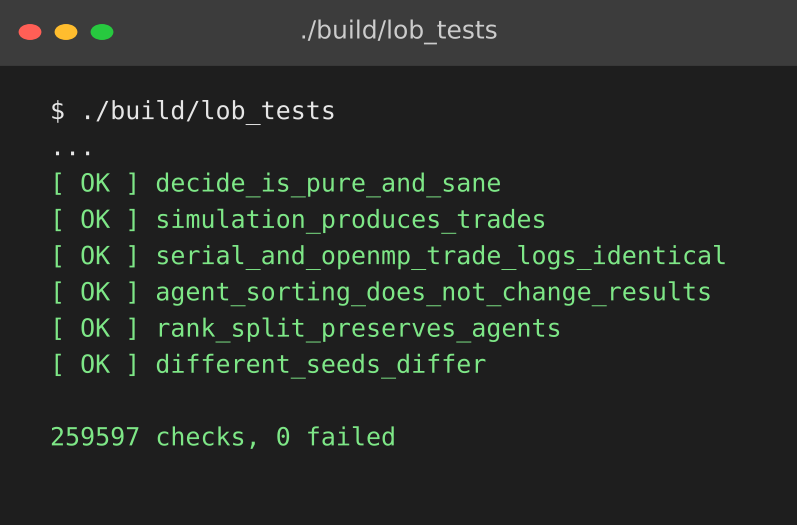
\includegraphics[width=0.8\columnwidth]{exec_tests.png}
\caption{Execution: unit test run (end of output).}
\label{fig:exec-tests}
\end{figure}

\begin{figure}[t]
\centering
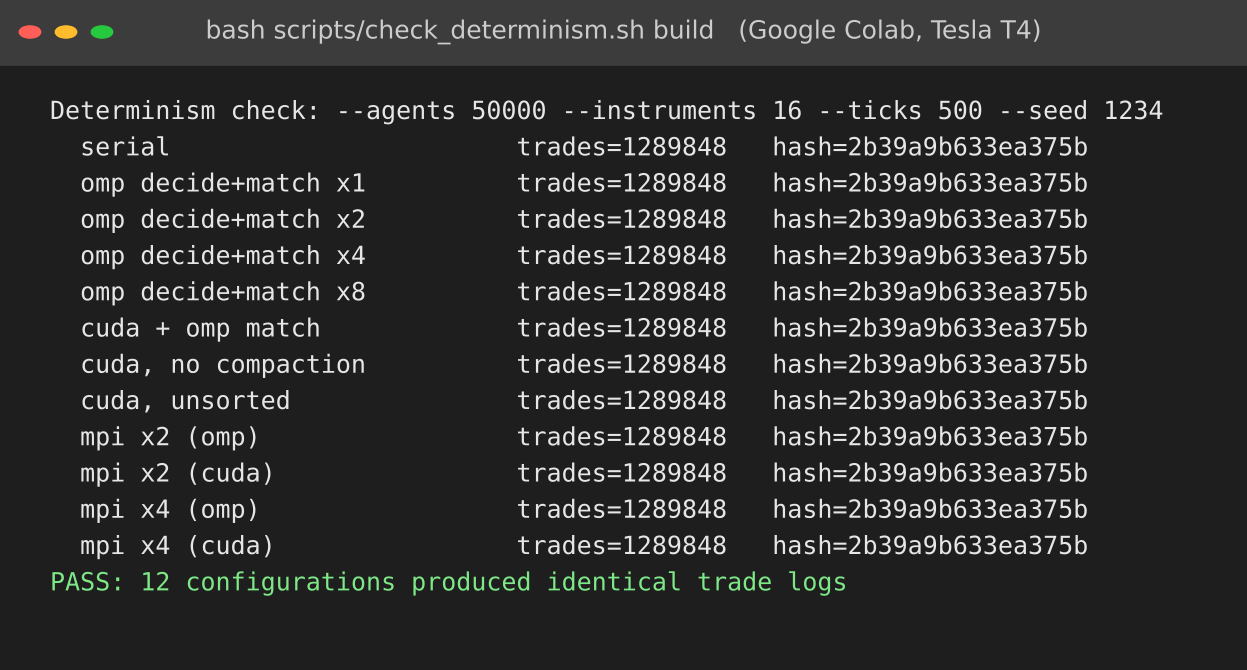
\includegraphics[width=\columnwidth]{exec_determinism_colab.png}
\caption{Execution on the Tesla T4: determinism check across 12 back-end configurations (output of
\texttt{scripts/check\_determinism.sh}).}
\label{fig:exec-det}
\end{figure}

\begin{figure}[t]
\centering
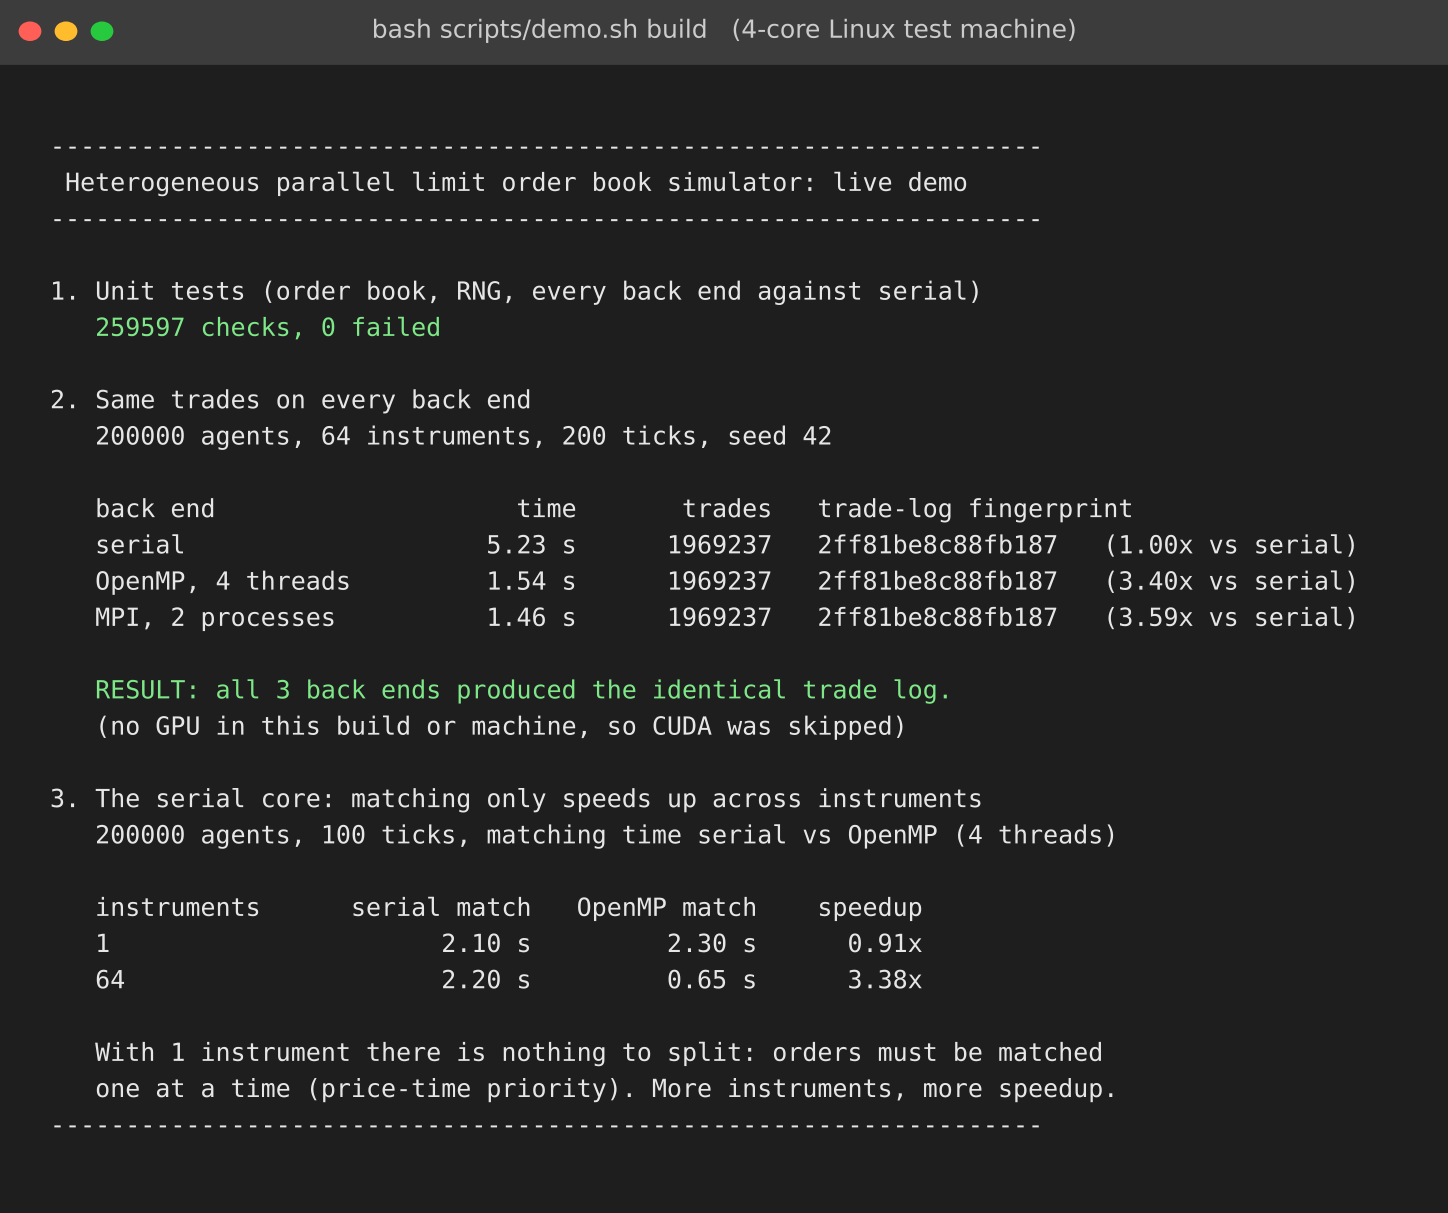
\includegraphics[width=\columnwidth]{exec_demo.png}
\caption{Execution: the live demo (\texttt{bash scripts/demo.sh build}) on a 4-core Linux machine
with 200{,}000 agents, 64 instruments and 200 ticks. Serial, OpenMP and MPI produce the same
1{,}969{,}237 trades and fingerprint; the last table shows that matching speeds up with 64
instruments but not with one.}
\label{fig:exec-demo}
\end{figure}

\begin{figure}[t]
\centering
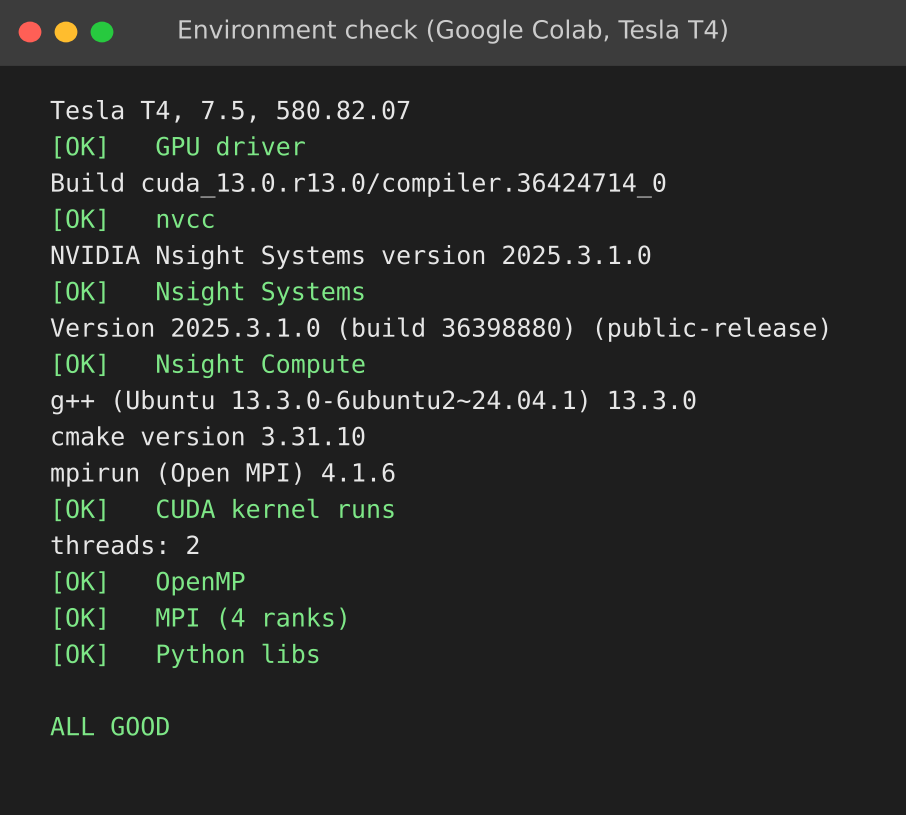
\includegraphics[width=0.75\columnwidth]{exec_colab_env.png}
\caption{Execution: Colab GPU environment check (CUDA 13, Nsight, Open MPI, OpenMP).}
\label{fig:exec-env}
\end{figure}

\subsection{GPU results (Tesla T4)}\label{sec:res-gpu}
Table~\ref{tab:phase} breaks one tick down at 1M agents and 128 instruments. The CUDA kernel takes
0.16\,ms against 13.7\,ms for two CPU threads, about 85$\times$ faster, but the decision phase as a
whole is only 3.6$\times$ faster: copying results back and scattering them into the agent array on
the host cost more than the kernel. Matching is unchanged at 84\,ms, so the whole tick improves
only from 97.4 to 87.9\,ms.

\begin{table}[t]
\centering
\caption{Time per tick by phase, 1M agents, 128 instruments (T4).}
\label{tab:phase}
\footnotesize
\begin{tabular}{@{}lrr@{}}
\toprule
Phase & OpenMP (2 thr.) & CUDA\\
\midrule
Agent decisions & 13.7 ms & 3.8 ms\\
\quad kernel & -- & 0.16 ms\\
\quad copy back (compacted) & -- & 0.46 ms\\
\quad host scatter & -- & $\approx$3.2 ms\\
Matching (CPU, OpenMP) & 83.7 ms & 84.1 ms\\
\midrule
\textbf{Whole tick} & \textbf{97.4 ms} & \textbf{87.9 ms}\\
\bottomrule
\end{tabular}
\end{table}

Fig.~\ref{fig:crossover} and Table~\ref{tab:crossover} show how CUDA compares with the OpenMP
baseline as the number of agents grows. Below about 4{,}000 agents CUDA is slower: copies and
kernel launches are a fixed cost, and copies alone are 30\% of the tick at 1{,}000 agents. CUDA
overtakes OpenMP between 4{,}000 and 16{,}000 agents and peaks at 1.41$\times$. Beyond that the
gain shrinks again, because matching grows with the number of orders and swallows the GPU's saving.

\begin{table}[t]
\centering
\caption{CUDA speedup over OpenMP (2 threads) and CPU--GPU copy share of tick time, 128 instruments.}
\label{tab:crossover}
\footnotesize
\setlength{\tabcolsep}{3.5pt}
\begin{tabular}{@{}lrrrrrrr@{}}
\toprule
Agents & 1k & 4k & 16k & 64k & 256k & 1M & 2M\\
\midrule
Speedup & 0.64 & 1.00 & \textbf{1.41} & 1.33 & 1.17 & 1.11 & 1.11\\
Copy share & 30.2\% & 13.6\% & 6.0\% & 2.3\% & 1.0\% & 0.6\% & 0.5\%\\
\bottomrule
\end{tabular}
\end{table}

\begin{widefigure}
\centering
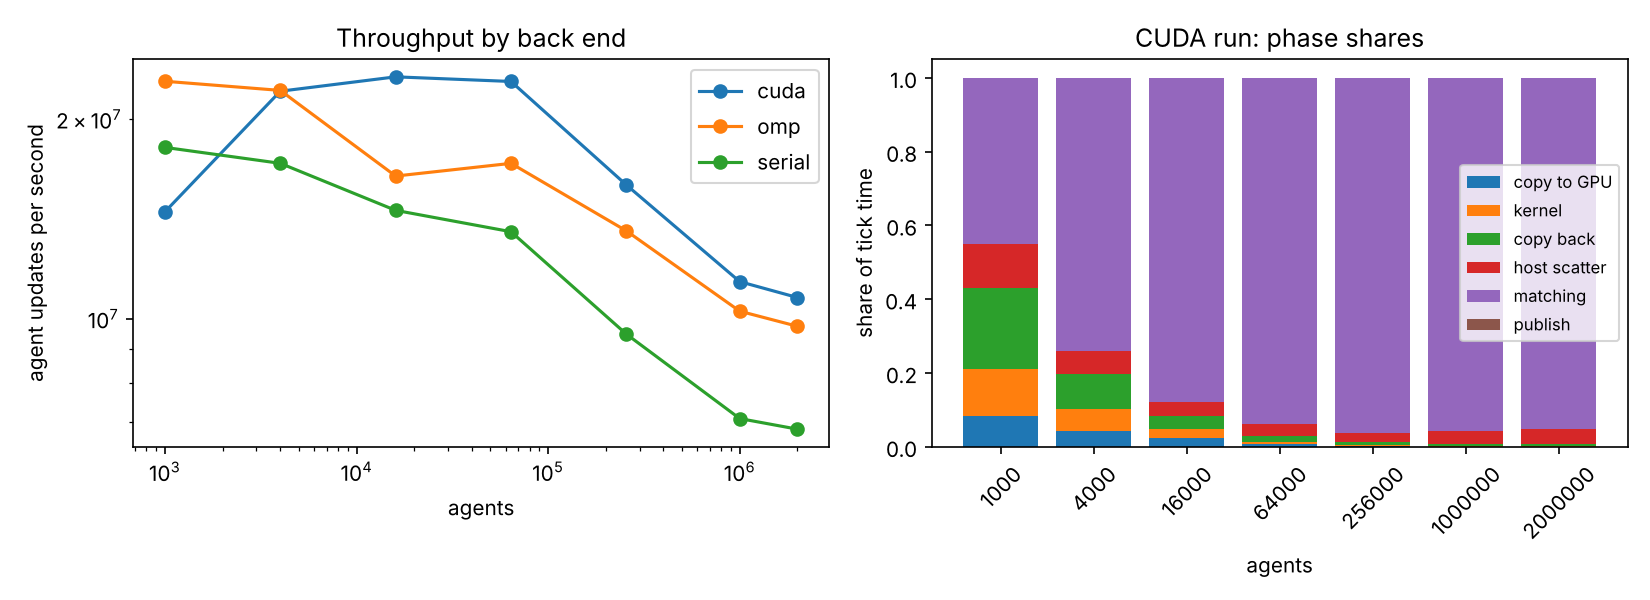
\includegraphics[width=\textwidth]{crossover.png}
\caption{CPU vs GPU crossover on the T4. Left: throughput (agent updates per second) of each back
end. Right: share of tick time per phase in the CUDA runs; matching dominates beyond 16k agents.}
\label{fig:crossover}
\end{widefigure}

Table~\ref{tab:kernel} and Fig.~\ref{fig:cuda} summarise the kernel experiments. Sorting agents by
strategy raises the number of active threads per warp instruction from 16.7 to 22.8 (32 means no
divergence), a 27\% reduction in divergence, and makes the kernel about 7\% faster. Compacting the
copy back to only the agents that acted cuts it from 1.90 to 0.46\,ms per tick (4.1$\times$). Block
sizes from 64 to 256 threads perform within 0.06\,ms of each other; 128 is best.

\begin{table}[t]
\centering
\caption{CUDA kernel metrics (Nsight Compute, 1M agents).}
\label{tab:kernel}
\footnotesize
\begin{tabular}{@{}lrr@{}}
\toprule
Metric & Sorted & Unsorted\\
\midrule
Active threads per warp instr. (of 32) & \textbf{22.8} & 16.7\\
Kernel duration & \textbf{0.138 ms} & 0.149 ms\\
Achieved occupancy & 82\% & 85\%\\
Registers per thread & 27 & 27\\
DRAM bandwidth & 173 GB/s & 168 GB/s\\
\midrule
Copy back, full / compacted & \multicolumn{2}{c}{1.90 ms / 0.46 ms}\\
\bottomrule
\end{tabular}
\end{table}

\begin{widefigure}
\centering
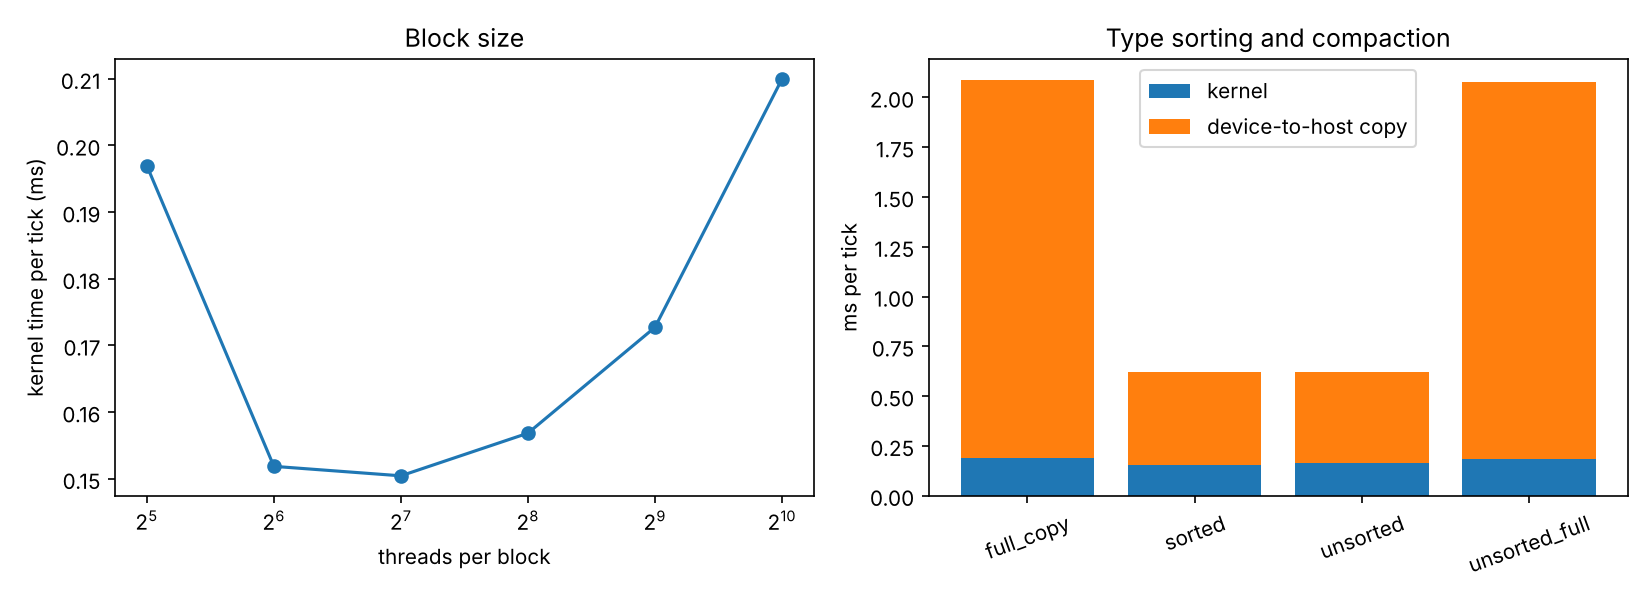
\includegraphics[width=\textwidth]{cuda_experiments.png}
\caption{CUDA kernel experiments. Left: kernel time per tick against block size. Right: kernel and
device-to-host copy time with and without type sorting and compaction.}
\label{fig:cuda}
\end{widefigure}

\subsection{CPU results (16-thread laptop)}\label{sec:res-cpu}
\textbf{Matching across instruments.} Table~\ref{tab:instr} and Fig.~\ref{fig:instr} show the
speedup of OpenMP matching over serial matching as instruments are added, with 16 threads. With one
instrument OpenMP is slightly \emph{slower} (0.90$\times$): there is nothing to split, so the only
effect is overhead. Speedup grows only as instruments are added, reaching 3.97$\times$ at 128.

\begin{table}[t]
\centering
\caption{OpenMP matching speedup over serial vs number of instruments (200k agents, 16 threads).}
\label{tab:instr}
\footnotesize
\setlength{\tabcolsep}{3.5pt}
\begin{tabular}{@{}lrrrrrrrr@{}}
\toprule
Instruments & 1 & 2 & 4 & 8 & 16 & 32 & 64 & 128\\
\midrule
Speedup & 0.90 & 0.97 & 1.97 & 2.14 & 2.63 & 3.23 & 3.54 & \textbf{3.97}\\
\bottomrule
\end{tabular}
\end{table}

\begin{figure}[t]
\centering
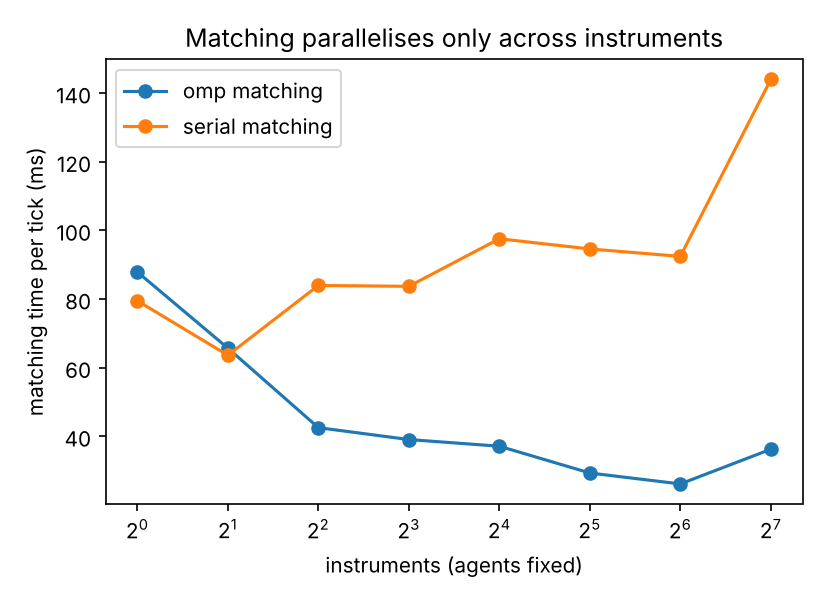
\includegraphics[width=0.85\columnwidth]{instruments.png}
\caption{Matching speedup grows only with the number of instruments.}
\label{fig:instr}
\end{figure}

\textbf{Strong scaling.} Table~\ref{tab:strong} and Fig.~\ref{fig:strong} show the whole simulation
with a fixed problem. Speedup peaks at 1.99$\times$ on 8 threads and falls to 1.74$\times$ on 16.
The decision phase, which needs no coordination between agents, improves only 1.75$\times$ on 8
threads (2.30\,s to 1.31\,s).

\begin{table}[t]
\centering
\caption{Strong scaling (400k agents, 64 instruments, 300 ticks, median of 5).}
\label{tab:strong}
\footnotesize
\setlength{\tabcolsep}{4pt}
\begin{tabular}{@{}lrrrrrr@{}}
\toprule
Threads $p$ & serial & 1 & 2 & 4 & 8 & 16\\
\midrule
Time (s) & 17.4 & 17.2 & 14.3 & 9.8 & 8.7 & 10.0\\
Speedup $S$ & 1.00 & 1.01 & 1.21 & 1.78 & \textbf{1.99} & 1.74\\
Efficiency $E$ & 1.00 & 1.01 & 0.61 & 0.45 & 0.25 & 0.11\\
Karp--Flatt $e$ & -- & -- & 0.65 & 0.42 & 0.43 & 0.55\\
\bottomrule
\end{tabular}
\end{table}

\begin{widefigure}
\centering
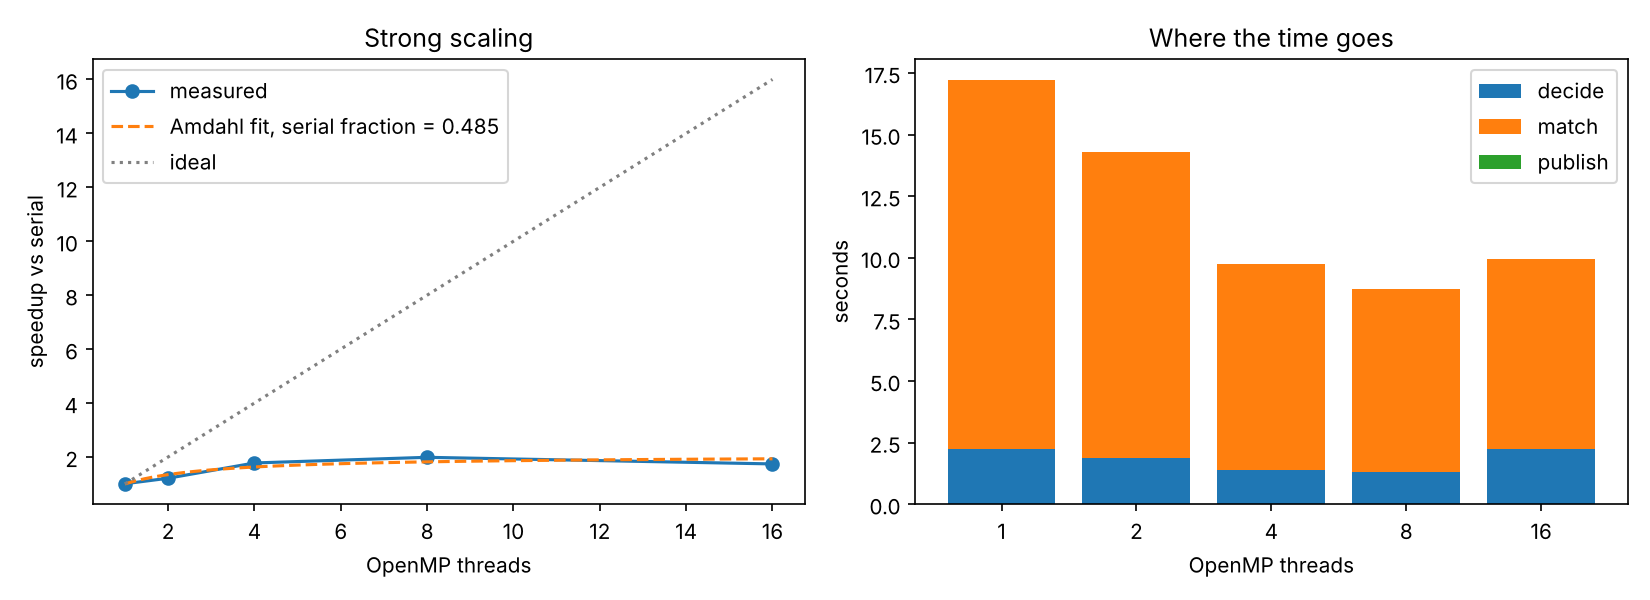
\includegraphics[width=\textwidth]{strong_scaling.png}
\caption{Strong scaling on the laptop. Left: measured speedup, Amdahl fit (serial fraction 0.485)
and ideal. Right: time per phase; matching dominates at every thread count.}
\label{fig:strong}
\end{widefigure}

\textbf{Weak scaling.} With 50{,}000 agents and 8 instruments per thread
(Table~\ref{tab:weak}, Fig.~\ref{fig:weak}), time should stay constant under ideal scaling. Instead,
efficiency falls to 0.11 at 16 threads, and total throughput levels off at about 11 million agent
updates per second, 1.8$\times$ the single-thread rate.

\begin{table}[t]
\centering
\caption{Weak scaling (50k agents and 8 instruments per thread, median of 5).}
\label{tab:weak}
\footnotesize
\begin{tabular}{@{}lrrrrr@{}}
\toprule
Threads & 1 & 2 & 4 & 8 & 16\\
\midrule
Time (s) & 2.40 & 3.62 & 6.27 & 11.07 & 21.85\\
Efficiency & 1.00 & 0.69 & 0.40 & 0.22 & 0.11\\
Updates/s (M) & 6.3 & 8.3 & 9.6 & 10.8 & 11.0\\
\bottomrule
\end{tabular}
\end{table}

\begin{figure}[t]
\centering
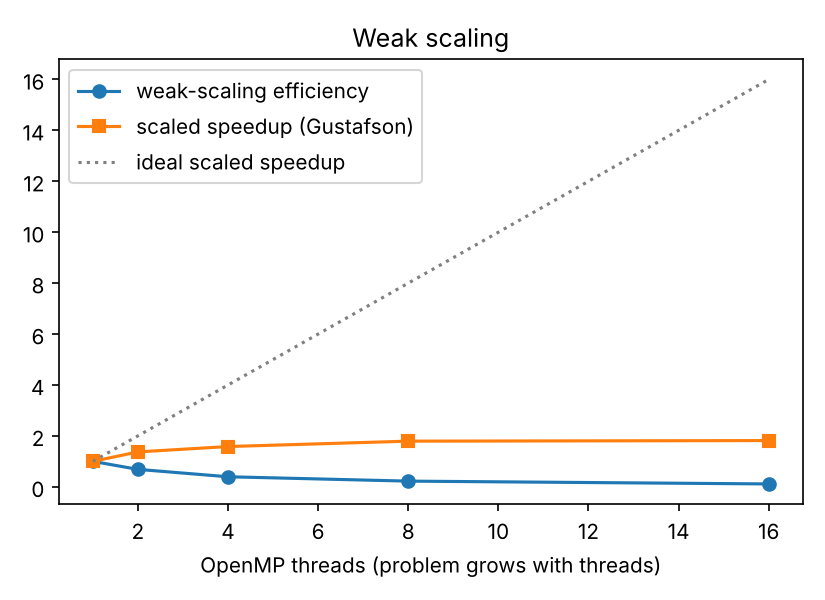
\includegraphics[width=0.85\columnwidth]{weak_scaling.png}
\caption{Weak scaling efficiency on the laptop.}
\label{fig:weak}
\end{figure}

\textbf{MPI.} With 400{,}000 agents and 64 instruments split over 1, 2 and 4 ranks on the same
machine (Fig.~\ref{fig:mpi}), communication plus waiting at the per-tick barrier takes 0\%, 20\%
and 39\% of tick time respectively. The message itself is one 64-bit integer; almost all of this
time is ranks waiting for the slowest rank, so it measures load imbalance more than message cost.
Total time barely changes, because the ranks share the same cores.

\begin{figure}[t]
\centering
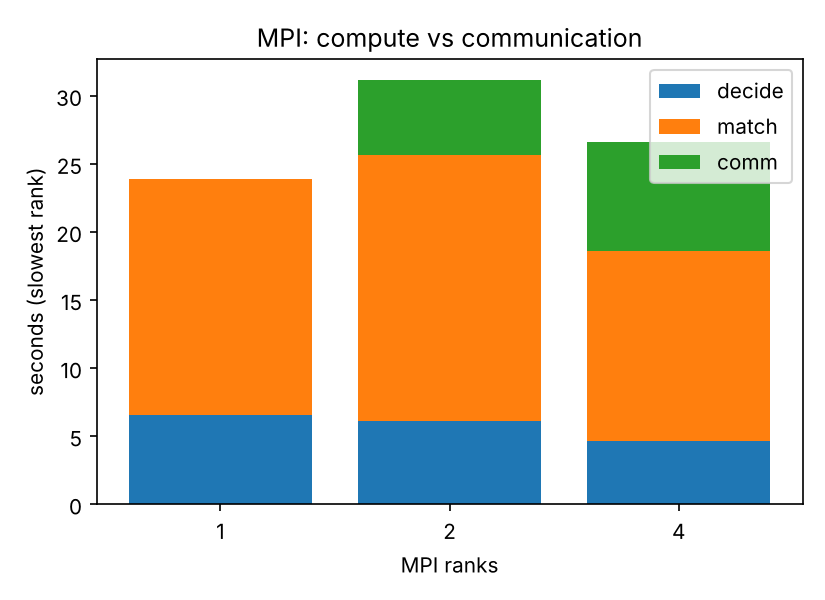
\includegraphics[width=0.85\columnwidth]{mpi.png}
\caption{MPI: share of tick time spent in communication and barrier wait.}
\label{fig:mpi}
\end{figure}

\textbf{False sharing.} With per-thread counters padded to separate cache lines, matching took
22.0\,ms per tick; unpadded, 20.8\,ms. The difference is within run-to-run noise: each thread
updates the counters only a few times per instrument per tick, so cache-line contention is too rare
to show. We report this as a negative result.

\subsection{Model realism}\label{sec:res-facts}
Table~\ref{tab:facts} and Fig.~\ref{fig:facts} compare the simulated returns with the stylised facts
of real markets~\cite{cont2001}. The model reproduces heavy tails and volatility clustering. It
fails the absence of linear autocorrelation: prices partly bounce back after a move (lag-1
autocorrelation $-0.33$), an effect of the mean-reverting and market-making agents.

\begin{table}[t]
\centering
\caption{Stylised facts of simulated 10-tick returns (16 instruments, 20k ticks).}
\label{tab:facts}
\footnotesize
\begin{tabularx}{\columnwidth}{@{}X r c@{}}
\toprule
Property (real markets) & Measured & Pass\\
\midrule
Heavy tails (excess kurtosis $> 0$) & 4.26 & yes\\
Volatility clustering ($|r|$ ACF lag 1 / lag 10 $> 0$) & 0.20 / 0.09 & yes\\
No linear autocorrelation (ACF lag 1 $\approx 0$) & $-0.33$ & no\\
Hill tail index (real: about 3--5) & 8.0 & partly\\
\bottomrule
\end{tabularx}
\end{table}

\begin{widefigure}
\centering
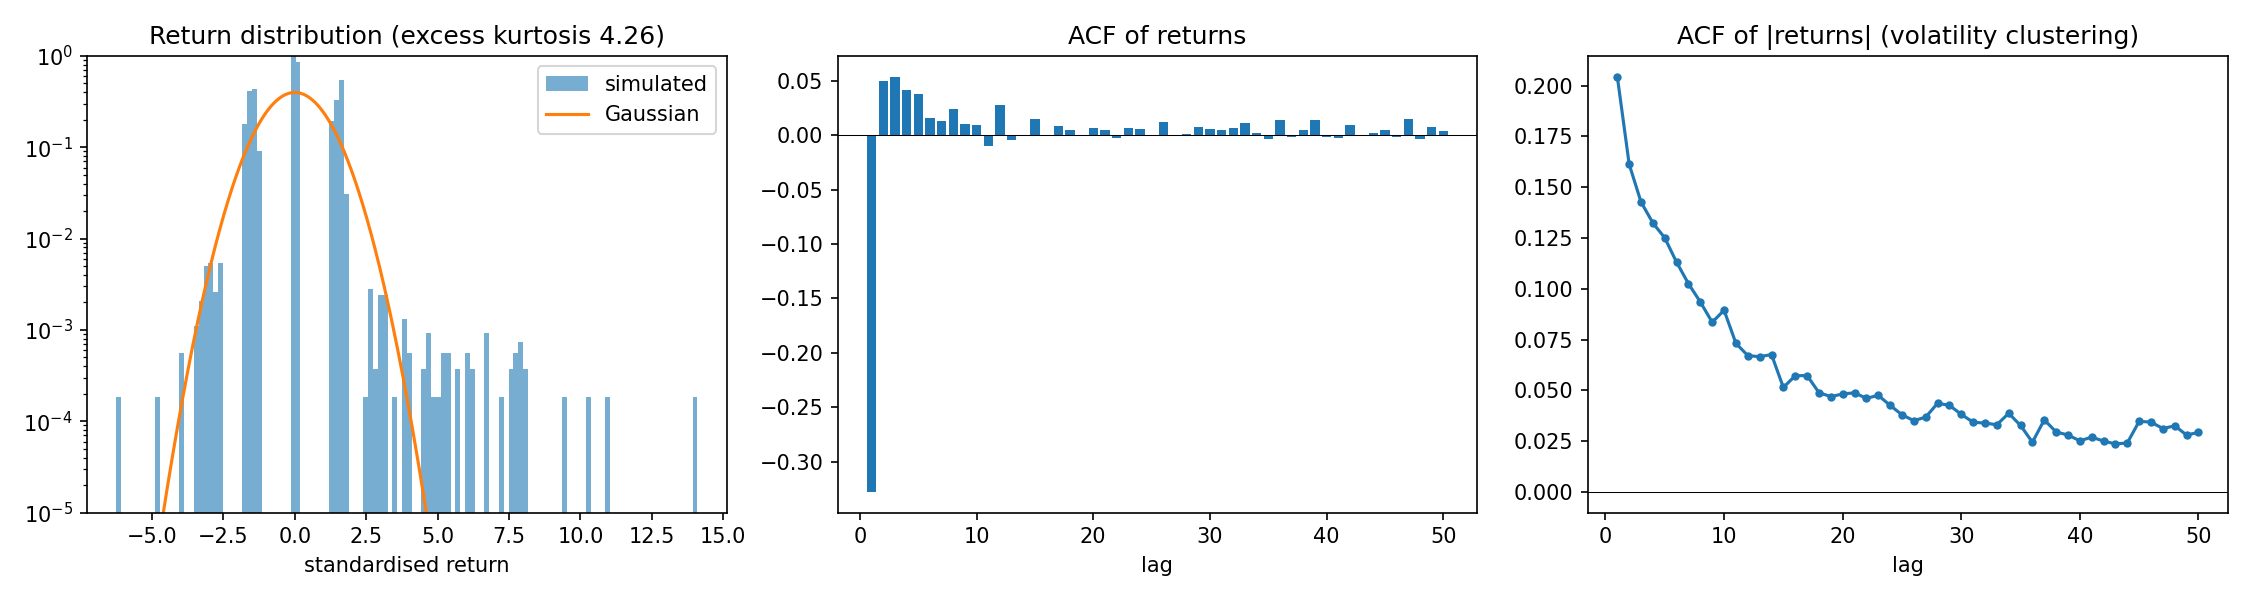
\includegraphics[width=\textwidth]{stylized_facts.png}
\caption{Stylised facts of simulated returns: return distribution against a Gaussian,
autocorrelation of returns and of absolute returns.}
\label{fig:facts}
\end{widefigure}

\section{Performance Analysis}\label{sec:perf}

\subsection{Speedup and efficiency}
Table~\ref{tab:speedups} collects the speedups. The pattern is the same everywhere: the parts that
are parallel over agents speed up well (85$\times$ for the kernel), while anything that includes
matching is limited to between 1.1$\times$ and 4$\times$. Parallel efficiency is high only at low
thread counts: 0.61 at 2 threads and 0.25 at 8 threads in strong scaling.

\begin{table}[t]
\centering
\caption{Summary of speedups.}
\label{tab:speedups}
\footnotesize
\begin{tabularx}{\columnwidth}{@{}X r@{}}
\toprule
Comparison & Speedup\\
\midrule
CUDA kernel vs 2-thread OpenMP decisions (1M agents) & 85$\times$\\
CUDA decision phase incl.\ copies and scatter & 3.6$\times$\\
Copy back, compacted vs full & 4.1$\times$\\
Kernel, type-sorted vs unsorted & 1.07$\times$\\
CUDA tick vs OpenMP tick (best, 16k agents) & 1.41$\times$\\
CUDA tick vs serial tick (32k--2M agents) & 1.54--1.61$\times$\\
OpenMP matching, 128 vs 1 instrument (16 threads) & 3.97$\times$ vs 0.90$\times$\\
Whole simulation, 8 threads (strong scaling) & 1.99$\times$\\
Demo run, 4-core machine: OpenMP / MPI (2 ranks) & 3.40$\times$ / 3.59$\times$\\
\bottomrule
\end{tabularx}
\end{table}

\subsection{Amdahl's law: where the bound comes from}
On the T4, the decision phase is 14\% of the OpenMP tick at 1M agents. Even an infinitely fast GPU
could then give at most $1/(1-0.14) \approx 1.16\times$; we measure 1.11$\times$, close to that
bound. The GPU has made decisions almost free, and matching is 92--96\% of every CUDA tick
(Fig.~\ref{fig:gustafson}). This is the Amdahl bound predicted in the synopsis: matching inside one
instrument is serial, and no GPU can remove it.

On the laptop, fitting Amdahl's law to the strong-scaling speedups gives an effective serial
fraction of $f=0.49$, which caps speedup at about $1/f \approx 2.1\times$. The Karp--Flatt values
(0.42--0.65) are of the same size and do not fall with $p$, so the limit is not simple parallel
overhead. The code's own serial work (publishing the index) takes about 0.001\,s of 17\,s, far too
little to explain $f$. Since even the coordination-free decision phase improves only 1.75$\times$
on 8 threads, we infer that the laptop's shared resources set the limit: a power-limited mobile
CPU lowers each core's clock as more cores become busy, and all cores share one memory bus, to
which matching (hash lookups and pointer chasing) is especially sensitive. This interpretation is
inferred from the timing pattern, not measured with hardware counters. The fitted $f$ is therefore
best read as an \emph{effective} serial fraction: serial code plus hardware saturation.

\subsection{Gustafson's law}
Gustafson's law predicts that growing the problem with the machine keeps efficiency high. On the
T4, growing agents at 32 fixed instruments keeps the CUDA speedup over serial at 1.54--1.61$\times$
from 32k to 2M agents (Fig.~\ref{fig:gustafson}): the speedup does not grow, because more agents
also mean more orders to match. On the laptop, weak-scaling efficiency drops to 0.11 at 16 threads
and throughput levels off at 1.8$\times$ the single-thread rate. Gustafson's law assumes that the
parallel part keeps scaling with more cores; that only holds while memory bandwidth and the power
budget also grow.

\begin{figure}[t]
\centering
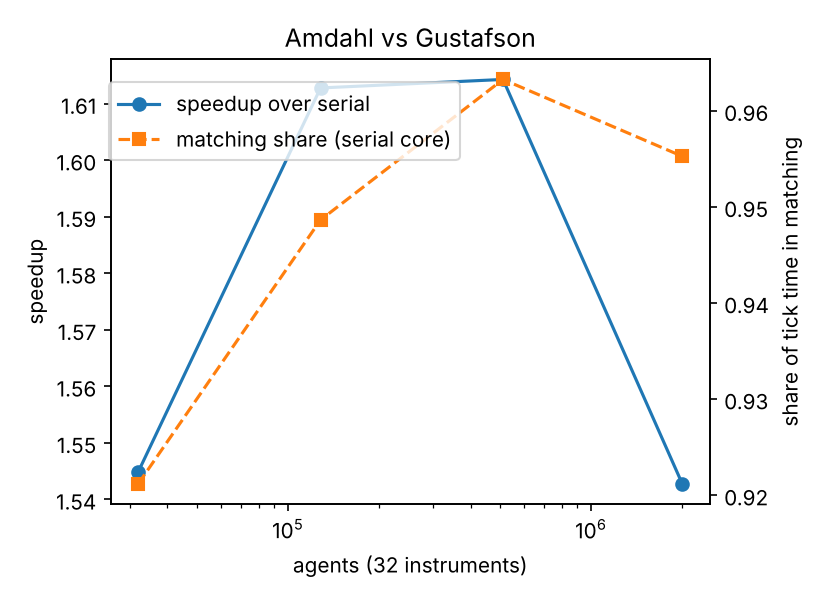
\includegraphics[width=0.85\columnwidth]{gustafson.png}
\caption{Growing agents at 32 fixed instruments on the T4: CUDA speedup over serial and matching
share of tick time.}
\label{fig:gustafson}
\end{figure}

\subsection{Roofline}
The decision kernel performs 3.95 integer operations per byte of DRAM traffic, below the T4's
ridge point of 12.7 (4.07\,Tops/s peak over 320\,GB/s), so it is memory-bound
(Fig.~\ref{fig:roofline}). It reaches 173\,GB/s, 54\% of peak bandwidth, at 82\% occupancy with 27
registers per thread. Further kernel tuning could at most halve a phase that is already under 1\% of
tick time, so it would not change the end-to-end result.

\begin{figure}[t]
\centering
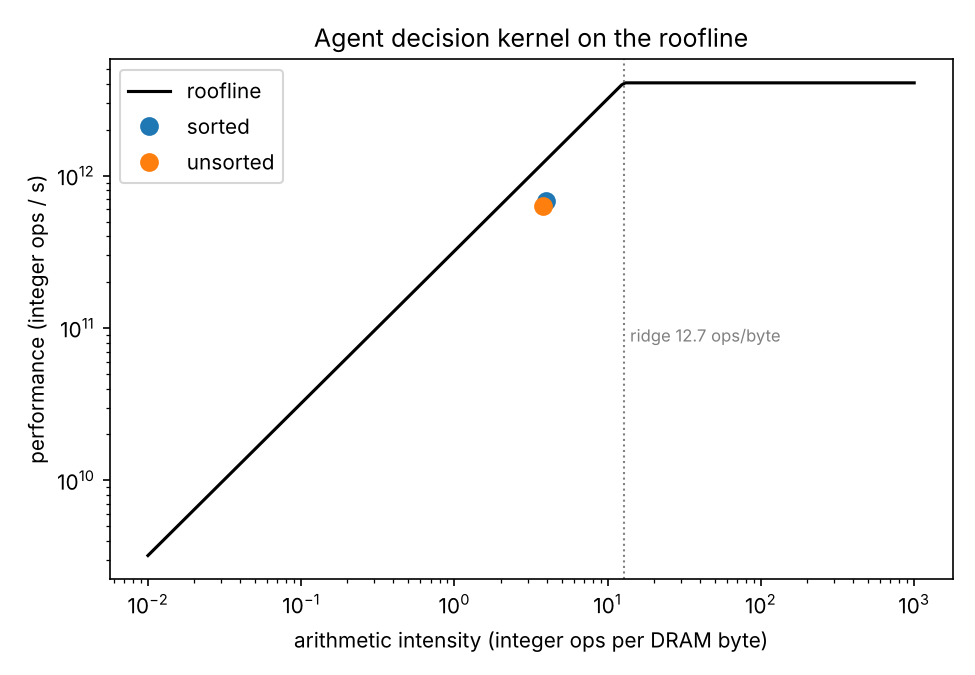
\includegraphics[width=0.85\columnwidth]{roofline.png}
\caption{Roofline placement of the decision kernel on the Tesla T4 (integer operations).}
\label{fig:roofline}
\end{figure}

\subsection{CPU vs GPU threshold}
Heterogeneous execution beats the multicore CPU when the GPU's saving on decisions exceeds the
fixed cost of the CPU--GPU boundary (two copies, a launch and the host scatter). On the T4 this
happens between 4{,}000 and 16{,}000 agents. The advantage then shrinks with size, because the
matching time that the GPU cannot touch grows with the number of orders. The threshold also depends
on the CPU: with more CPU threads, OpenMP decisions are faster, so the GPU needs more agents to pay
off. Finally, the host scatter (about 3.2\,ms at 1M agents) costs 20 times the kernel; moving more
of the pipeline to the GPU would only pay if matching moved too, which price--time priority
prevents within an instrument.

\subsection{Bottleneck summary}
\begin{itemize}
\item \textbf{Matching} under price--time priority is the bottleneck on every back end: 92--96\% of
  a CUDA tick, and it parallelises only across instruments.
\item \textbf{The CPU--GPU boundary} (copies and host scatter) costs more than the kernel; compaction
  reduces it by 4.1$\times$.
\item \textbf{Hardware saturation} (power and memory bandwidth) limits CPU scaling to about
  2$\times$ on the laptop before the code's own serial part does.
\item \textbf{MPI} cost is dominated by load imbalance at the per-tick barrier, not by data volume.
\end{itemize}

% Sections 13-16: Comparison with Existing Methods, Conclusion, Future Scope. Shared by both templates.

\section{Comparison with Existing Methods}\label{sec:compare}
Table~\ref{tab:compare} positions this work against the closest existing systems. Direct speed
comparisons are not meaningful, because the systems simulate different models on different
hardware; we compare what each one parallelises, how it handles reproducibility, and what it
measures.

\begin{widetable}
\centering
\caption{This work compared with existing methods.}
\label{tab:compare}
\footnotesize
\begin{tabularx}{\textwidth}{@{}p{2.4cm} X X X X@{}}
\toprule
System & What runs in parallel & Matching & Reproducibility & Scaling analysis\\
\midrule
ABIDES / ABIDES-Gym~\cite{byrd2020abides,amrouni2021} & nothing (serial event loop) & serial, one exchange & seed only & none\\
JAX-LOB~\cite{frey2023} & independent books on GPU & serial within book, on GPU & not discussed & per-message timing\\
PyMarketSim~\cite{mascioli2024} & nothing & serial, one asset & not discussed & single-thread throughput\\
FLAME GPU 2~\cite{richmond2023} & agents on GPU (spatial models) & not applicable (bidding sub-models) & atomics non-deterministic & agent-count scaling\\
Repast4Py~\cite{collier2022} & spatial partitions over MPI & not applicable & seed; cross-rank equality not addressed & strong scaling\\
SIMCoV-GPU~\cite{leyba2024} & spatial domains over GPUs & not applicable & statistical only ($\approx$1\%) & strong and weak scaling\\
\midrule
\textbf{This work} & agents on GPU or CPU cores; instruments over threads and MPI ranks & serial within instrument, parallel across instruments & \textbf{bit-identical trade log} on all back ends & strong, weak, Amdahl fit, Karp--Flatt, roofline, crossover\\
\bottomrule
\end{tabularx}
\end{widetable}

\textbf{Same conclusion, measured.} JAX-LOB states that matching inside one book is
serial~\cite{frey2023}. Our results quantify the consequence end to end: matching is 92--96\% of a
CUDA tick, so an 85$\times$ faster kernel yields only 1.1--1.6$\times$ for the whole simulation.

\textbf{Different decomposition.} Spatial ABM frameworks~\cite{richmond2023,collier2022,leyba2024}
partition by space and exchange halos. We partition by instrument, which removes all cross-rank
conflicts; the only per-tick communication is one integer reduction. The cost moves to load
imbalance at the barrier (20--39\% of tick time with 2--4 ranks), the analogue of Repast4Py's
communication-bound regime.

\textbf{Stronger reproducibility.} SIMCoV-GPU matches CPU and GPU results only
statistically~\cite{leyba2024}, and OpenRAND makes only the random numbers
reproducible~\cite{khan2024}. Counter-based random numbers, integer-only decisions, a deterministic
arrival order and order-independent compaction together give a bit-identical trade log across 12
configurations, so a parallel bug shows up as a changed fingerprint.

\textbf{Measured threshold.} Like SIMCoV-GPU, we find the GPU pays off only above a problem size;
we locate it at 4{,}000--16{,}000 agents against the 2-thread CPU and explain both the lower bound
(fixed copy and launch cost) and why the advantage shrinks again (growing matching time).

\textbf{Limits of this comparison.} Our CPU baseline on the T4 has only 2 threads; a stronger CPU
would move the crossover up. Our agents are simpler than ABIDES agents (no inventory or latency
model), and the model fails the no-autocorrelation stylised fact.

\section{Conclusion}\label{sec:concl}
We built a heterogeneous agent-based limit order book simulator with agent decisions in CUDA,
matching parallelised across instruments with OpenMP, and instruments distributed with MPI. All
eight objectives of the synopsis were met. Every back end produces a bit-identical trade log for a
given seed, which made correctness checkable throughout. The measurements give one consistent
answer: order matching under price--time priority is the scaling bottleneck. The GPU makes agent
decisions about 85$\times$ faster, yet the whole tick improves by at most 1.41$\times$ over the
CPU baseline, because matching takes 92--96\% of the time; the measured 1.11$\times$ at 1M agents
sits close to the Amdahl bound of 1.16$\times$. Matching parallelises only across instruments
(0.90$\times$ with one, 3.97$\times$ with 128). The GPU overtakes the multicore CPU between 4{,}000
and 16{,}000 agents, below which copy and launch costs dominate. On the laptop, CPU scaling levels
off near 2$\times$ (effective serial fraction 0.49) because of shared power and memory limits, and
MPI overhead is dominated by load imbalance at the per-tick barrier. The simulated returns show
heavy tails and volatility clustering, with excess short-term mean reversion as a known limitation.

\section{Future Scope}\label{sec:future}
\begin{itemize}
\item \textbf{Faster matching.} Match independent price levels speculatively, or batch orders in
  periodic call auctions, which allow parallel matching within an instrument at the cost of
  changing market rules.
\item \textbf{Moving the host scatter to the GPU.} Keep agent state and intents on the device and
  send per-instrument order lists directly, removing the 3.2\,ms host scatter.
\item \textbf{Load balancing for MPI.} Assign instruments to ranks by measured activity instead of
  contiguous blocks, to cut barrier waiting; and run on a real multi-node cluster to measure network
  cost.
\item \textbf{More realistic agents.} Add inventory, cash and latency, and tune the agent mix to
  remove the negative lag-1 autocorrelation.
\item \textbf{Stronger hardware study.} Repeat the crossover on a server CPU with many cores and on
  newer GPUs, and confirm the hardware-saturation explanation with performance counters.
\item \textbf{Multi-GPU.} Give each MPI rank its own GPU for very large agent populations.
\end{itemize}


\bibliographystyle{IEEEtran}
\bibliography{refs}
\end{document}
